\chapter{Enquadramento}
\label{cap2}

Este capítulo exemplifica a utilização de referências, figuras, tabelas e listagens.

\section{Projeto}
\par A Brisa solicitou a colaboração da Deloitte para o desenvolvimento de uma plataforma tecnologia que permita disponibilizar informação de gestão consolidada/agregada fazendo uso das suas base de dados de informação de gestão e fazendo uso exclusivo de tecnologias open-source. Desta forma, a Deloitte iniciou uma prestação de serviços com uma duração de 6 meses com a participação de uma equipa de dois recursos, com a minha participação durante três meses e com a supervisão de um gestor de projeto com vasta experiência em soluções de Business Intelligence. A equipa de projeto foi completada com a participação de dois gestores de projeto da Brisa. O planeamento do projeto foi definido fazendo uso de metodologias Agile por diferentes motivos, nomeadamente, a necessidade de concretizar ajuste rápidos ao nível tecnológicos e de arquitetura até a sua estabilização final e devido ao fato de estarmos a colaborar com o cliente na definição de indicadores e layout de dasboards e reports que permitam caraterizar o negócio da melhor forma.
\section{Objetivo}
\par No âmbito do estágio foi definido que a minha participação no projeto iria contemplar todas as fases e componentes do projeto, por forma, a ter uma perceção global e integrada de toda a plataforma. Esta abordagem permitiu ter a experiência de interagir diretamente com o cliente incluindo nas fases de definição de requisitos e de testes de aceitação. 
\par Como objectivo complementar ao projeto, mas não menos importante fui inserido numa equipa de desenvolvimento, com metodologias adequadas mercado de trabalho, contribuindo isto para o aumento das importantes soft-skils.
\section{Planeamento}
\par O projeto foi desenvolvido, como já referido, recorrendo a metodologias Agile. Foi distribuído por quatro fases de desenvolvimento distintas, com uma sequência de trabalhos associada a cada fase. Face ao planeamento inicial ocorreram alguns ajustes no decorrer do estágio para fazer face aos ajustamentos que o projeto careceu durante a sua fase de desenvolvimento, como podemos observar na Figura  \ref{fig:planeamentoFig}. 
\begin{figure}[!htb]
\centering
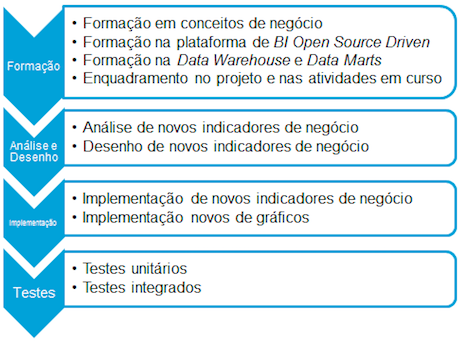
\includegraphics[width=9cm]{planeamento}
\caption{Planeamento}
\label{fig:planeamentoFig}
\end{figure}